% !TEX root = main.tex
\section{Time dependent fit}
\label{sec:Tfit}

This section covers the phasespace integrated, time-dependent fit to $\Bs\to\Ds\hadron\pion\pion$ data.
%For the phasespace integrated fit to $\Bs\to\Ds\kaon\pion\pion$ data, the sensitivity to the CKM phase $\gamma$ will depend on the magnitude of the coherence factor $\kappa$, defined in Eq. \ref{eq:coherenceFactor}, 
%which is added as an additional fit parameter. 
We use the \textsf{sFit} technique \cite{Pivk:2004ty}  to statistically remove background from the decay time fit, leaving only the signal PDF to describe the decay time. 
The \textsf{sWeights} are calculated based on the fit to the reconstructed $B_s$ mass distribution described in Sec.~\ref{sec:massFits}.
As additional input to the fit, the tagging information (Sec. \ref{sec:Tagging}), 
as well as the decay time acceptance (Sec. \ref{sec:Acceptance}) and resolution (Sec. \ref{sec:Resolution}) is used and fixed to the values obtained by the dedicated studies. 
Taking all inputs into account, the final time dependent fit PDF is given by
\begin{equation}
\label{eq:TPDF_full}
\mathcal{PDF}(t,\vec{\lambda}) = \left(\epsilon(t)\cdot \int P(x,t,q_t,q_f) \text d x \right) \times \mathcal{R}(t - t^{'}),
\end{equation}
where $\int P(x,t,q_t,q_f) \text d$ is the PDF given by Eq. \ref{eq:PDF_intX}, $\epsilon(t)$ is the efficiency due to the time acceptance effects and $\mathcal{R}(t - t^{'})$ is the Gaussian time resolution function. 



\subsection{sFit to $\Bs\to\Ds\pion\pion\pion$ data}  
The phasespace-integrated, time-dependent fit is performed to the full sWeighted sample of selected candidates from Run I and 2015+2016 Run II data, containing both possible magnet polarities and all $\Ds$ final states.
In the fit, the values of $\Gs$ and $\DGs$ are fixed to the latest PDG report \cite{PDG2016}. All tagging parameters are fixed to the central values found in the tagging calibration, described in Sec. \ref{sec:Tagging}.
Due to the fact that the $\Bs\to\Ds\pion\pion\pion$ decay is flavour specific, the CP-coefficients can be fixed to $C=1$ and $D_{f} = D_{\bar{f}} = S_{f} = S_{\bar{f}} = 0$, reducing Eq. \ref{eq:PDF_intX} to

\begin{equation}
\int P(x,t,q_t,q_f) \text d x = [\text{cosh} \left( \frac{\Delta \Gamma \, t}{2}\right) + q_t q_f \, \text{cos} \left( m_s \, t \right)] e^{- \Gamma t}.
\end{equation}

Note that in this case, the dependence on the coherence factor $\kappa$ is dropped and the same relation as found for $\Bs\to\Ds\pion$ decays is recovered. 
Therefore, the only free fit parameter left is $\dms$. The data distribution with the overlaid fit is shown in Fig. \ref{fig:tFitNorm}.

\begin{figure}[h]
	\centering
		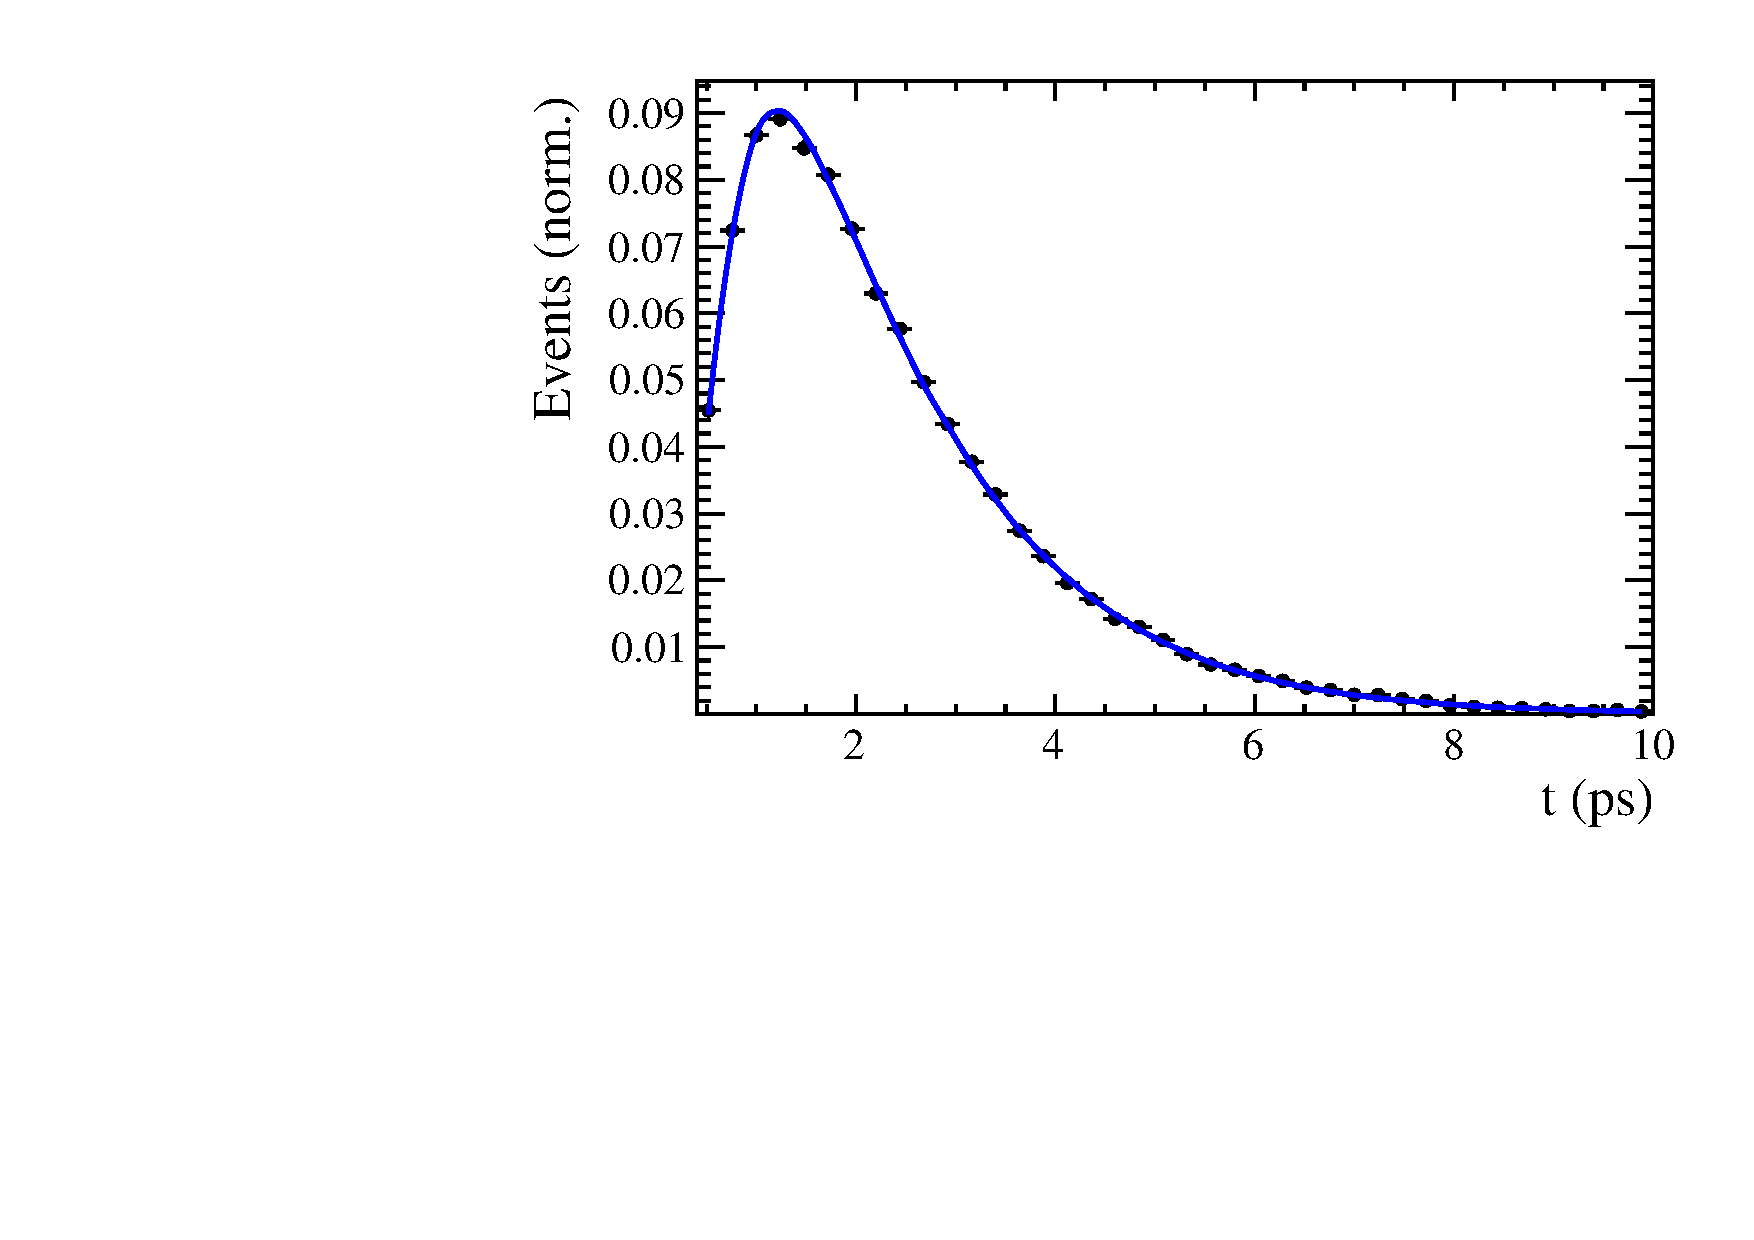
\includegraphics[width=0.45\textwidth, height = !]{figs/timeFit/norm_taggingCalib/h_t.pdf} 
		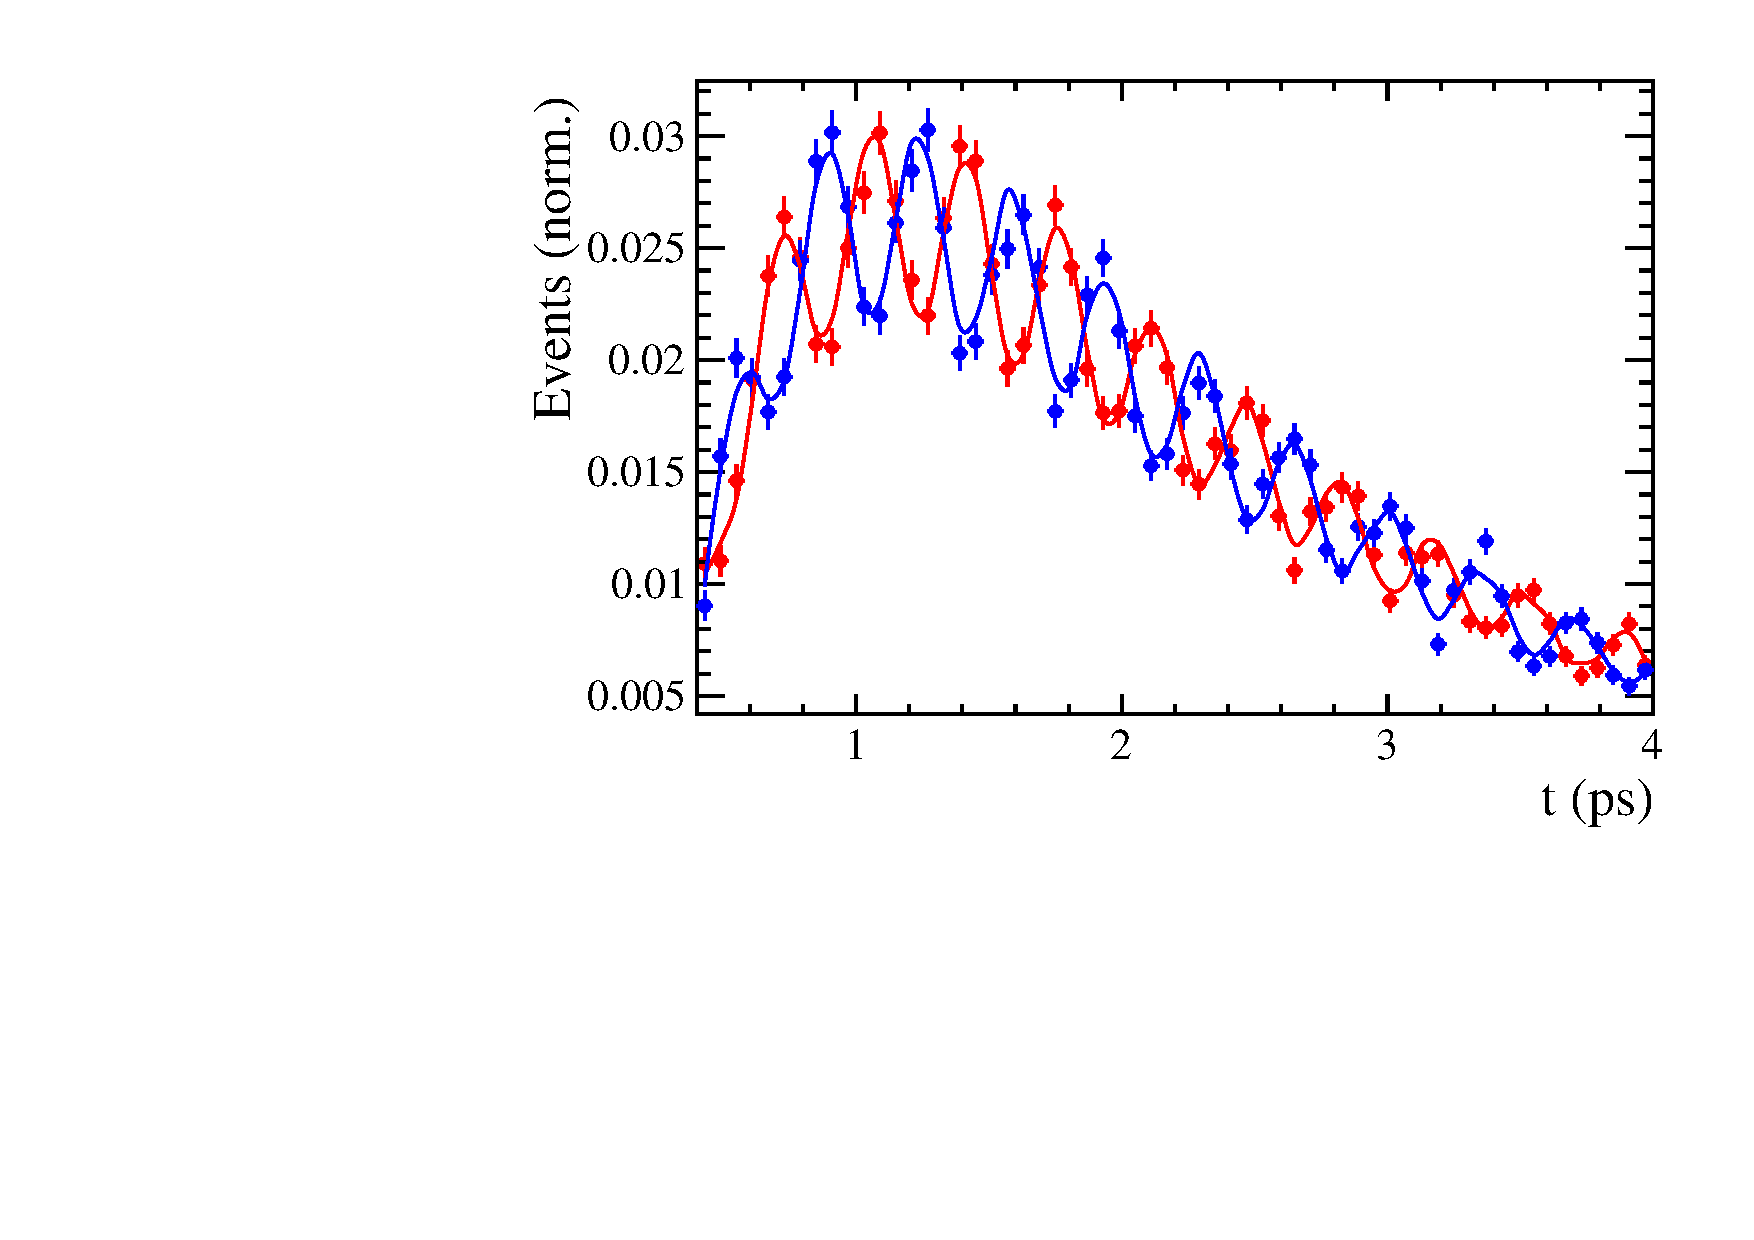
\includegraphics[width=0.45\textwidth, height = !]{figs/timeFit/norm_taggingCalib/h_t_mixed.pdf} 
		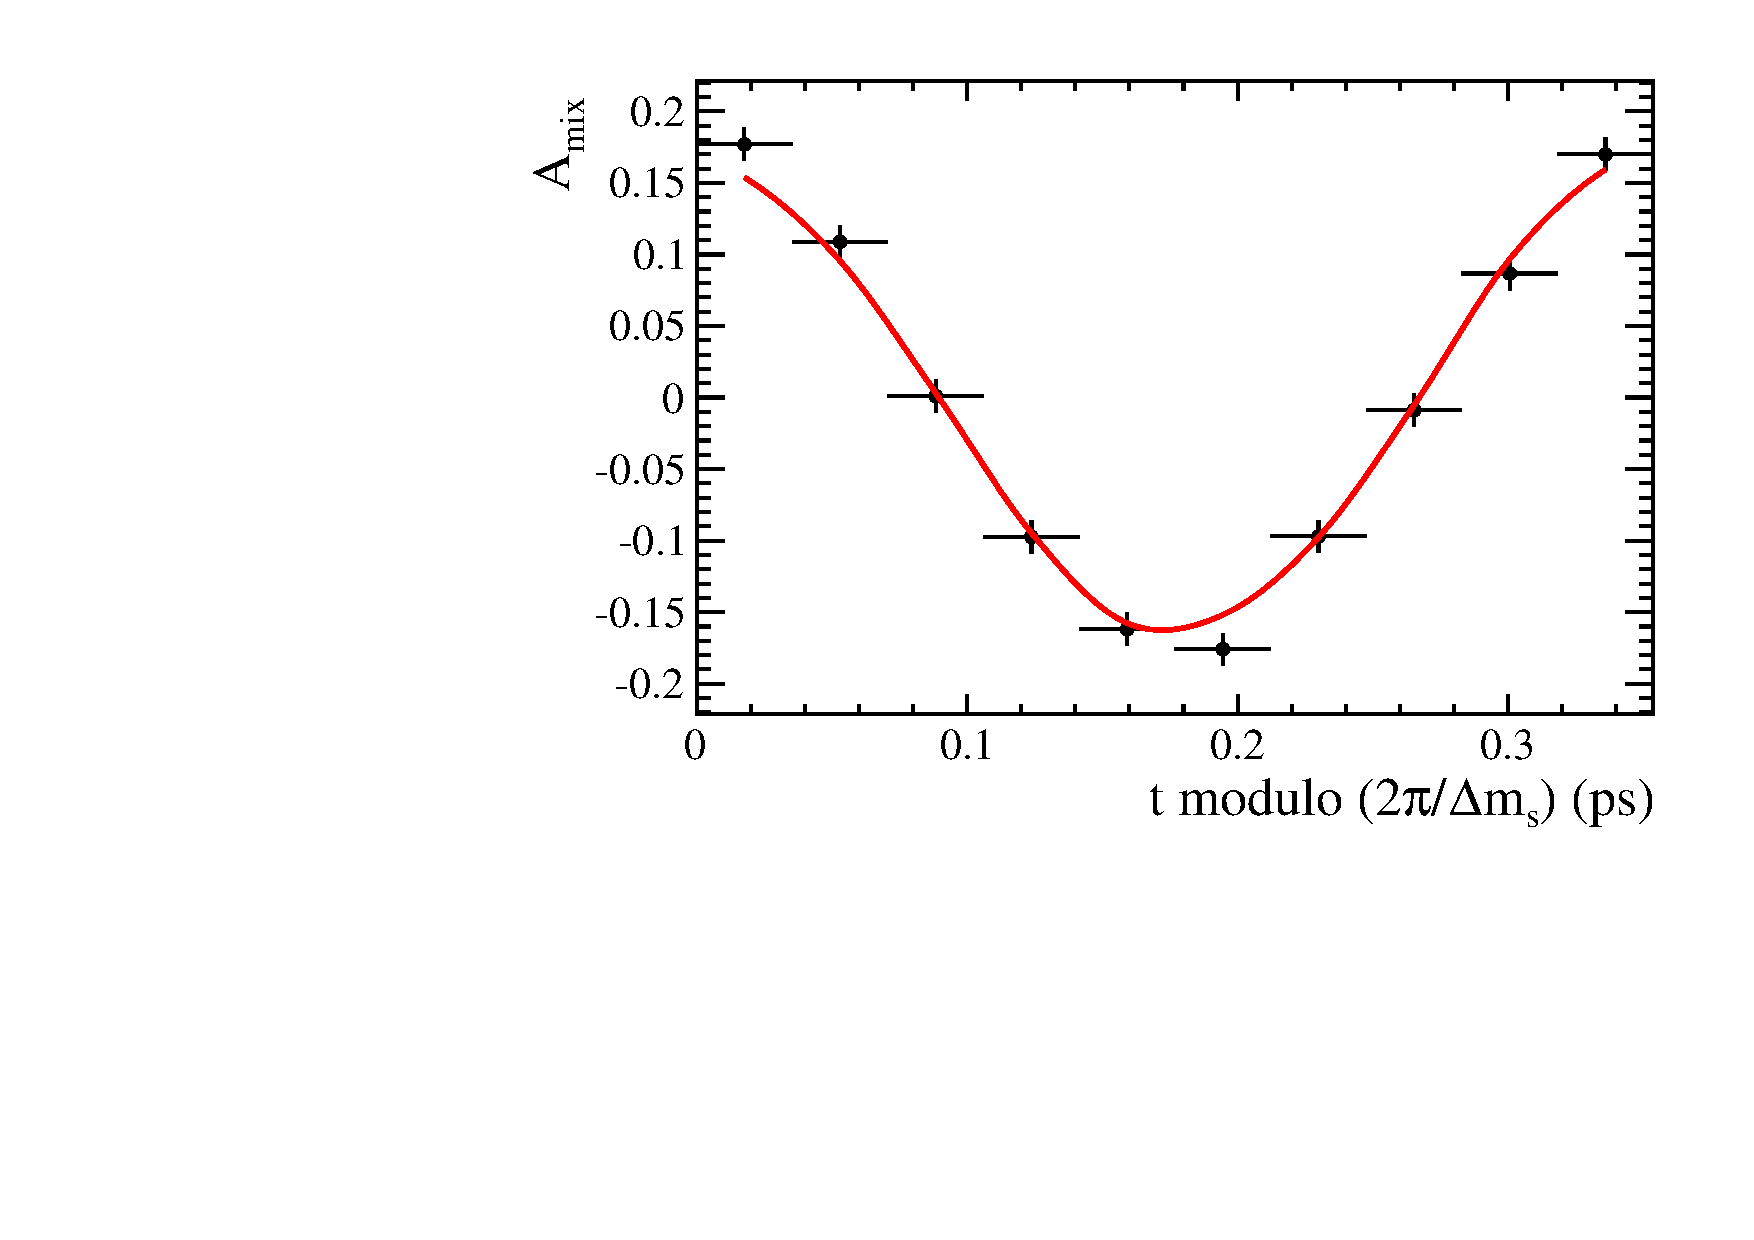
\includegraphics[width=0.45\textwidth, height = !]{figs/timeFit/norm_taggingCalib/h_asym.pdf} 		
		\caption{Top left: Flavour averaged decay time distribution of $\Bs\to\Ds\pion\pion\pion$ candidates with the averaged fit overlaid. 
Top right: Tagged decay time distribution of mixed (red) and unmixed (blue) signal candidates with the fit described in the text overlaid. 
Bottom: Time-dependent asymmetry $A_{mix}$ between mixed and unmixed $\Bs$ candidates in bins of $t/(2\pi\dms)$. A fit to this distribution using a $cos(t\cdot\dms)$ function is overlaid.} 		
		\label{fig:tFitNorm}
\end{figure}	

\begin{table}[h]
\centering
\caption{Result of the time-dependent amplitude fit to $B_s \to D_s K \pi \pi$ data.}
\begin{tabular}{c c}
\hline
\hline
Fit parameter & Value \\
\hline
$x_{-}$ &  xx.xx  $\pm$ 0.352\\
$y_{-}$ &  xx.xx  $\pm$ 0.159\\
$x_{+}$ &  xx.xx  $\pm$ 0.210\\
$y_{+}$ &  xx.xx  $\pm$ 0.162\\
\hline
\hline
\end{tabular}
\label{table:fullFit_signal}
\end{table}

\clearpage
\subsection{sFit to $\Bs\to\Ds\kaon\pion\pion$ data}
The time-dependent fit to the sWeighted sample of $\Bs\to\Ds\kaon\pion\pion$ signal candidates is performed simultaneously in the four bins defined in Sec. \ref{subsec: AccComparison}, 
spliting the data into Run I \& II and trigger category 0 (L0Hadron TOS) \& 1 (L0Hadron TIS). 
In these four bins, the respective description of the decay-time acceptance (Sec. \ref{sec:Acceptance}) is used as an input. 
As further input the decay-time resolution scaling relation, found separately for Run I \& II in Sec. \ref{sec:Resolution}, is used in the simultaneous fit. 
The full fit model is given in Eq. \ref{eq:TPDF_full}, where $\int P(x,t,q_t,q_f)$ is: 

\begin{equation} 
           \int P(x,t,q_t,q_f) \text d x \propto    [
        \, \text{cosh} \left( \frac{\Delta \Gamma \, t}{2}\right) 
          + q_t q_f \, C \, \text{cos} \left( m_s \, t \right)  
          + \kappa \, D_{q_f} \, \text{sinh} \left( \frac{\Delta \Gamma \, t}{2}\right)  
          - q_t \, \kappa \, S_{q_f}\, \text{sin} \left( m_s \, t \right)  ]  e^{- \Gamma t}.
\end{equation}

Note that the integration over the available phase space $x$ gives rise to the coherence factor $\kappa$, which dilutes the sensitivity to the CP coefficients $D$ \& $S$ and with that, also to the CKM phase $\gamma$. 
All input parameters from the tagging, time acceptance and resolution are fixed in the fit. The CP coefficients, as well as $\kappa$, are therefore the only parameters left floating. 
The data distribution and the overlaid fit is shown in Fig. \ref{fig:tFitSig}.


\begin{table}[h]
\centering
\caption{Result of the time-dependent amplitude fit to $B_s \to D_s K \pi \pi$ data.}
\begin{tabular}{c c}
\hline
\hline
Fit parameter & Value \\
\hline
$x_{-}$ &  xx.xx  $\pm$ 0.352\\
$y_{-}$ &  xx.xx  $\pm$ 0.159\\
$x_{+}$ &  xx.xx  $\pm$ 0.210\\
$y_{+}$ &  xx.xx  $\pm$ 0.162\\
\hline
\hline
\end{tabular}
\label{table:fullFit_signal}
\end{table}

\begin{figure}[h]
	\centering
		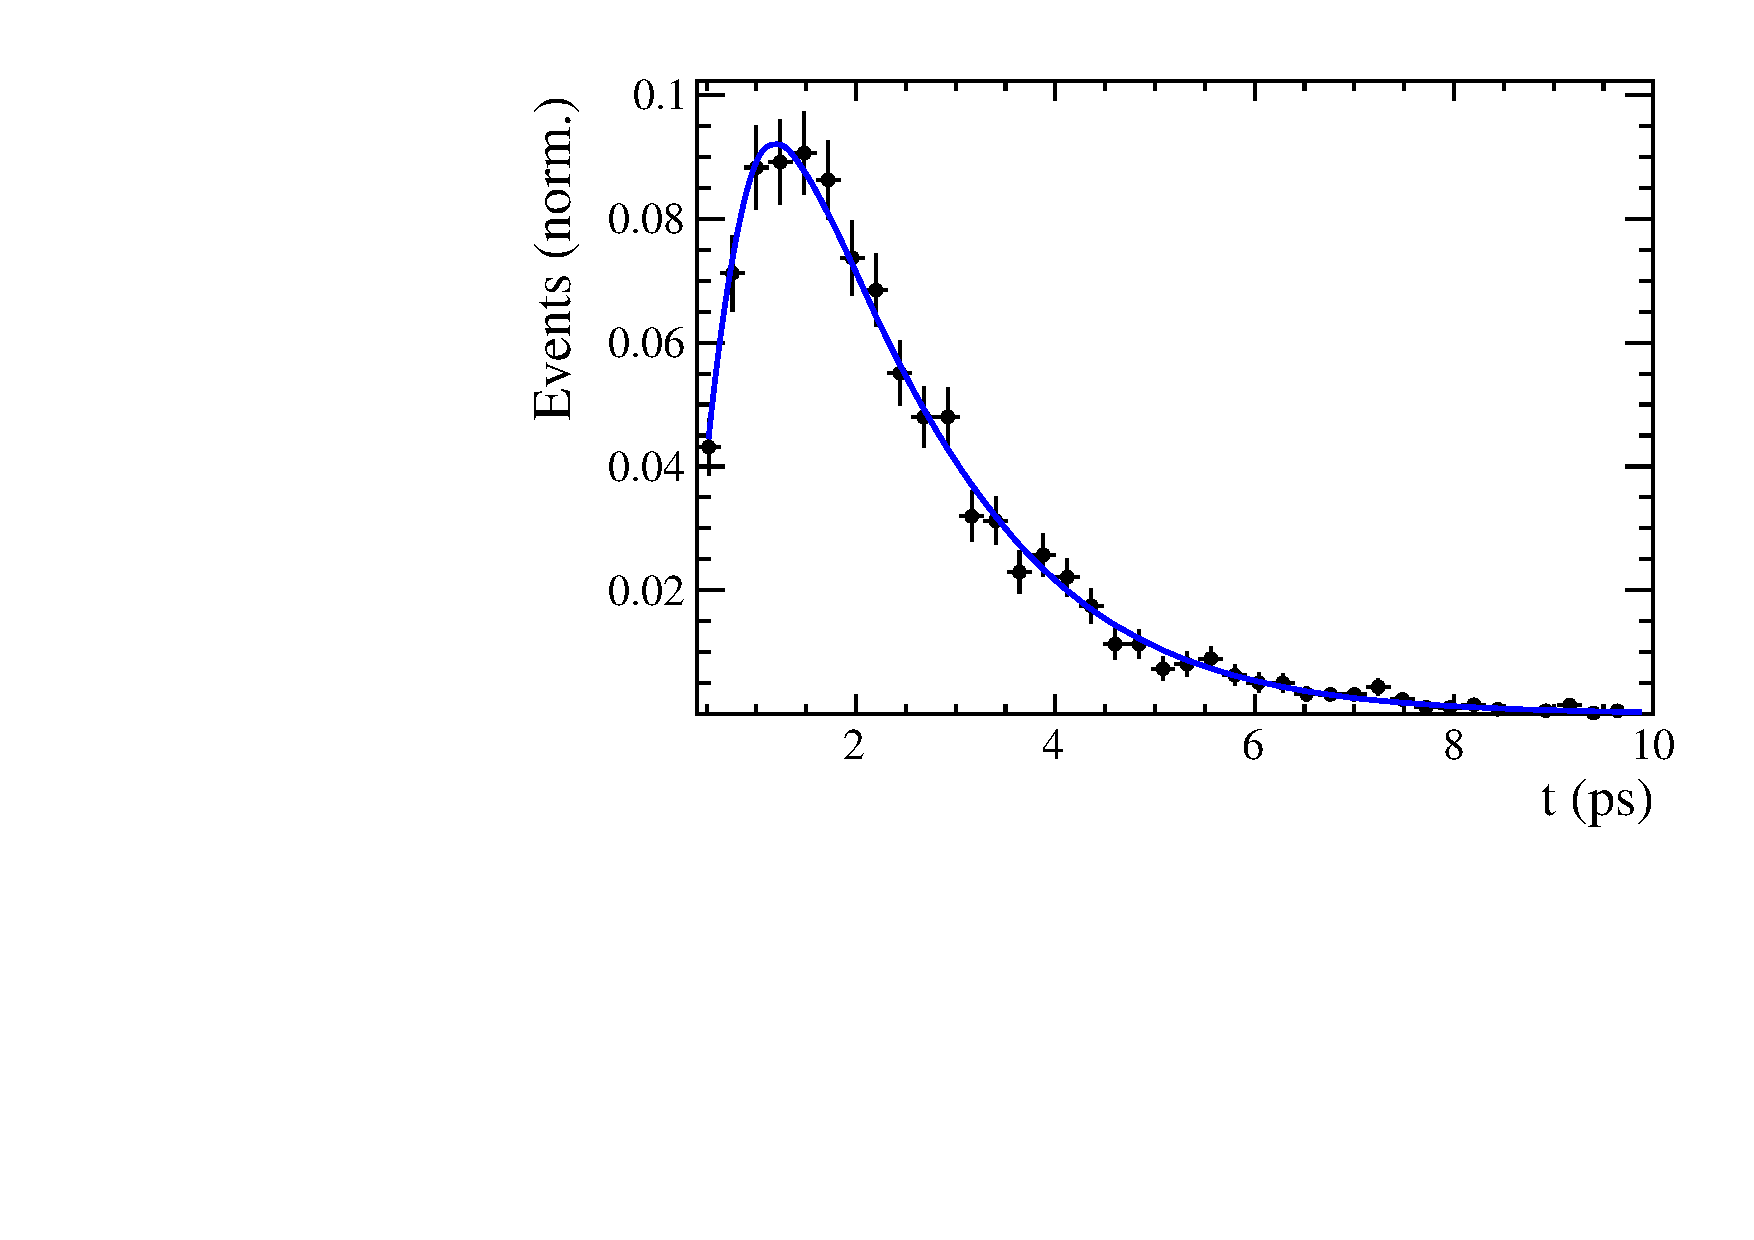
\includegraphics[width=0.45\textwidth, height = !]{figs/timeFit/signal/h_t.pdf} 
%		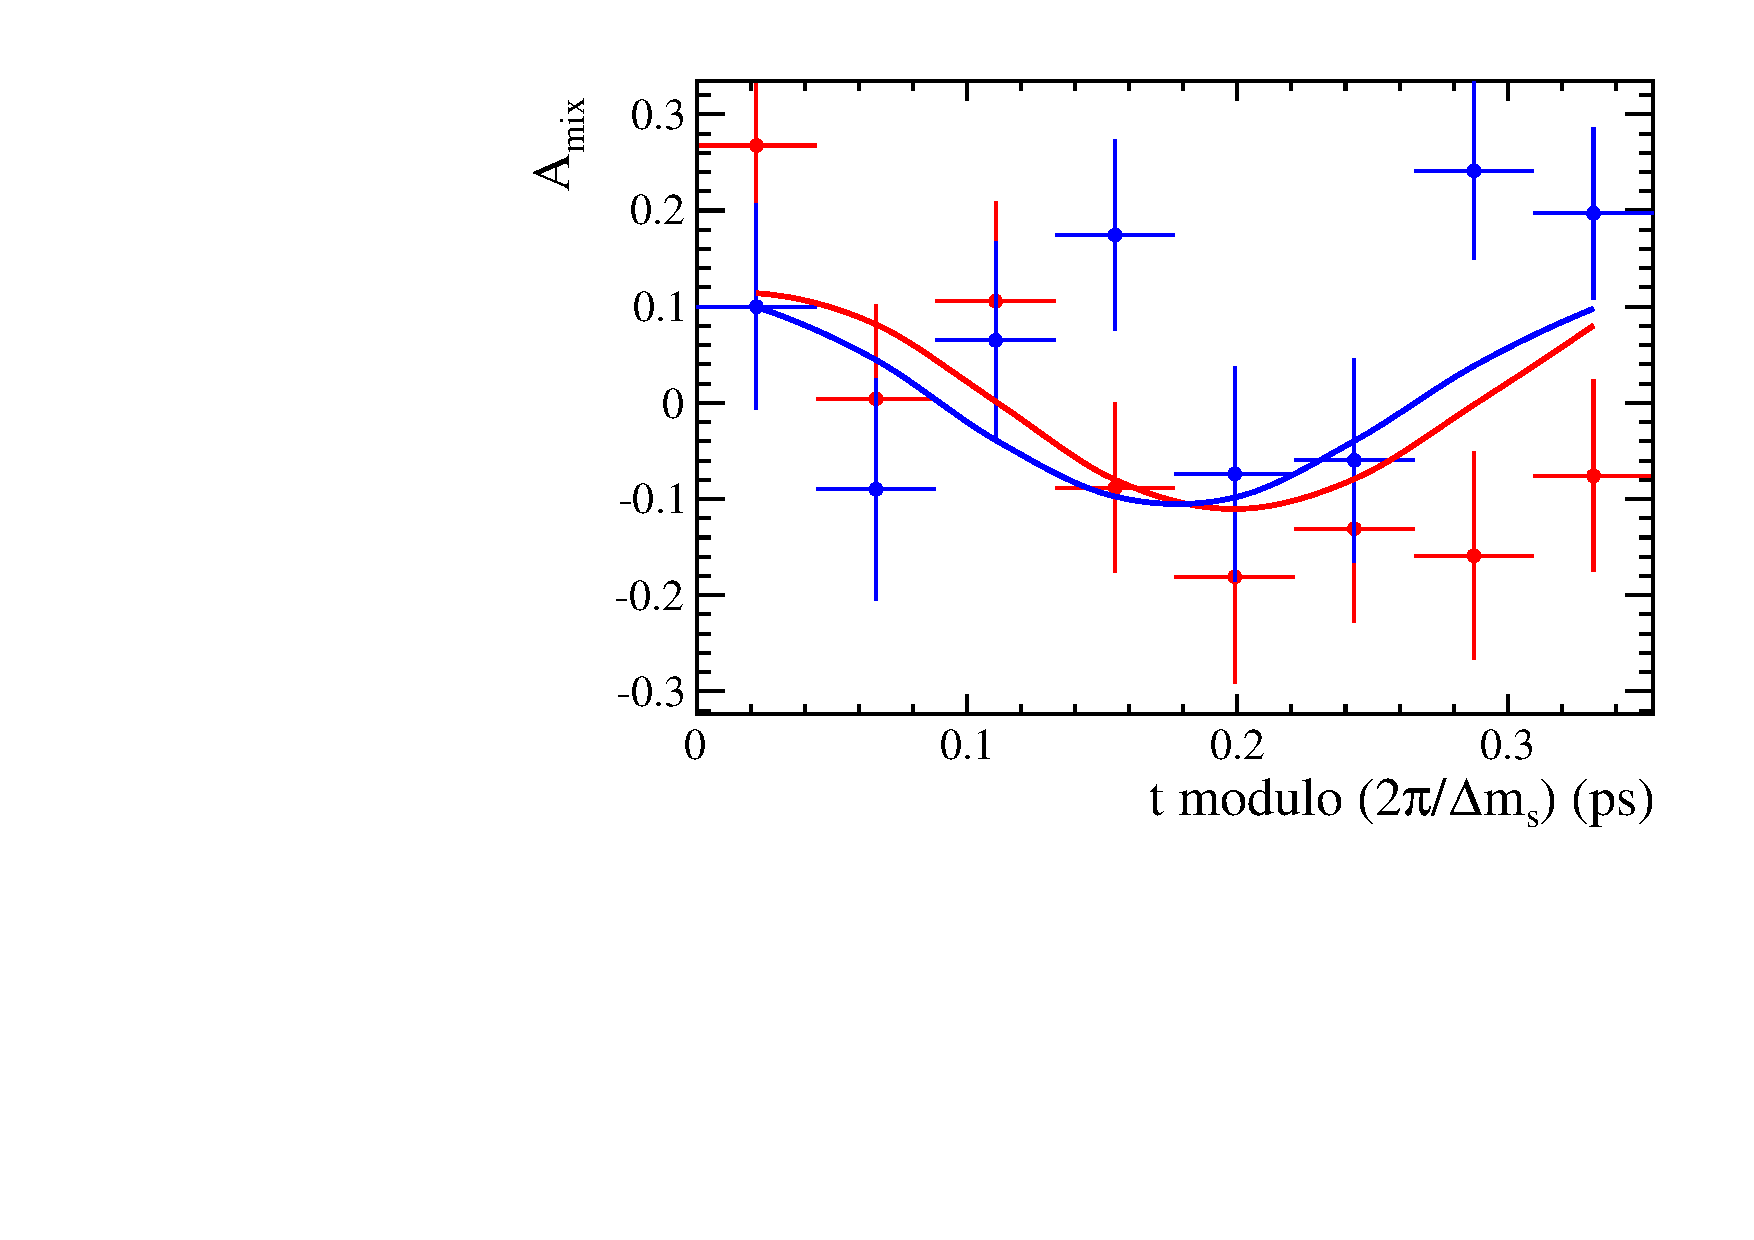
\includegraphics[width=0.45\textwidth, height = !]{figs/timeFit/signal/h_asym.pdf} 		
		\caption{Tagged and sWeighted decay-time distribution of $\Bs\to\Ds\kaon\pion\pion$ signal candidates. The fit described in the text is overlaid.} 
		\label{fig:tFitSig}
\end{figure}	


\subsection{\textsf{sFit} model validation using toy studies}
The fit model and procedure is validated using pseudo experiments. 1000 toys are generated using the model described in Eq. \ref{eq:TPDF_full} and \ref{eq:PDF_intX}. 
Each pseudo experiment is generated with the same amount of signal events found in the Run I + 2015/2016 data samples.  
Figure \ref{fig:ToyPulls_tdfit} shows the pull distributions for all CP coefficients, where every pull P of a parameter x is given as $P = \frac{x_{gen} - x_{fit}}{\Delta x}$.


\begin{figure}[h]
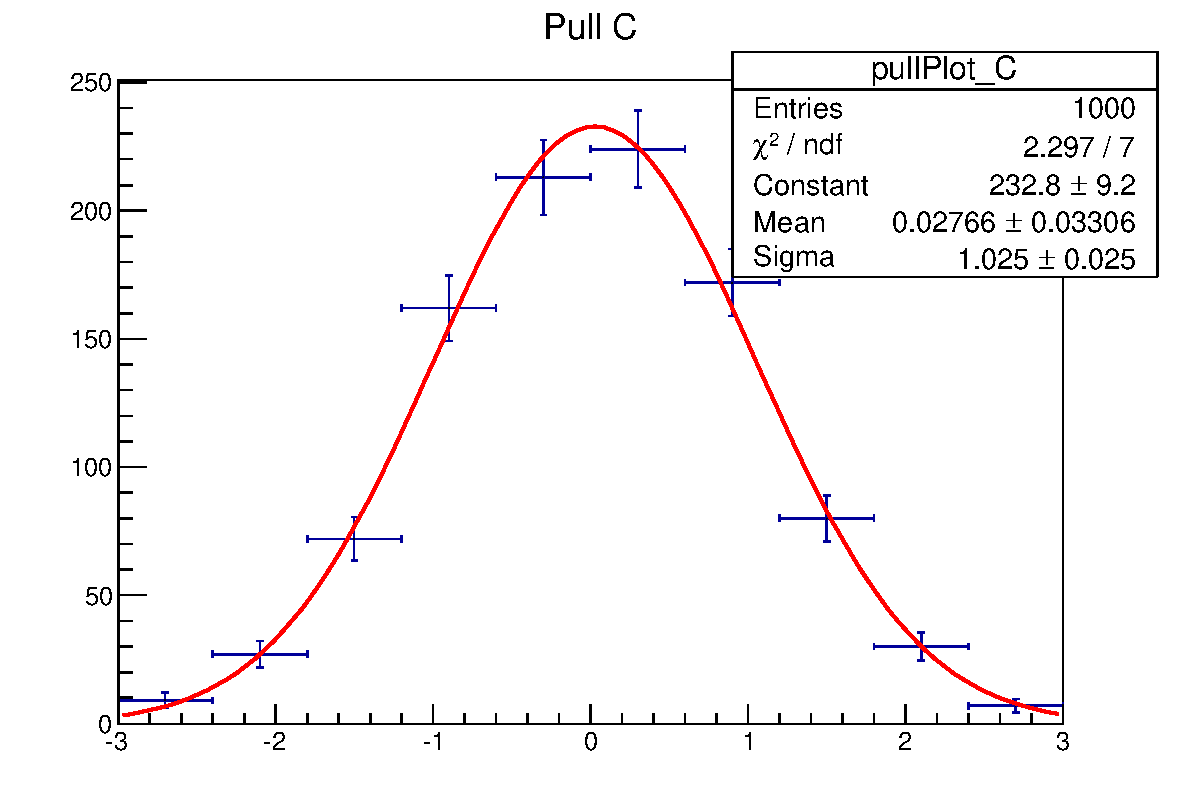
\includegraphics[height=!,width=0.49\textwidth]{figs/plots_toy/studies_timeFit/pull_C_all_Gaussfit.pdf}
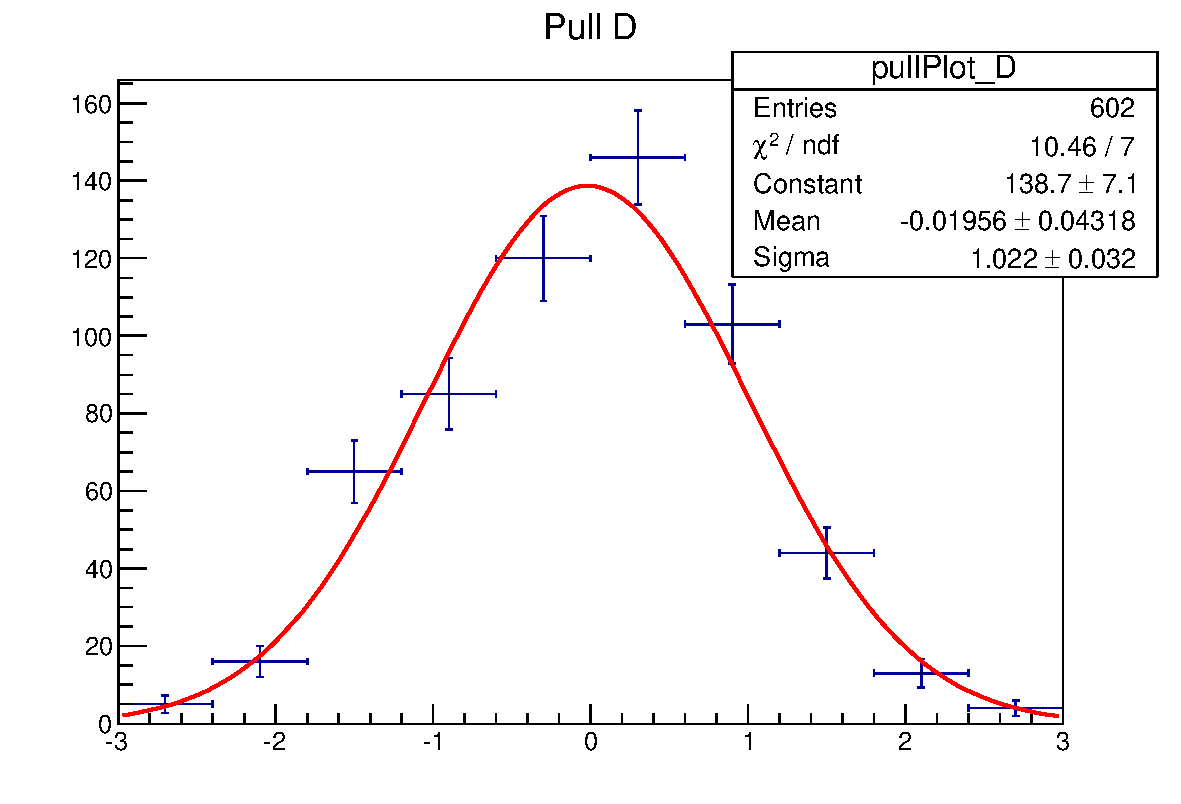
\includegraphics[height=!,width=0.49\textwidth]{figs/plots_toy/studies_timeFit/pull_D_all_Gaussfit.pdf}
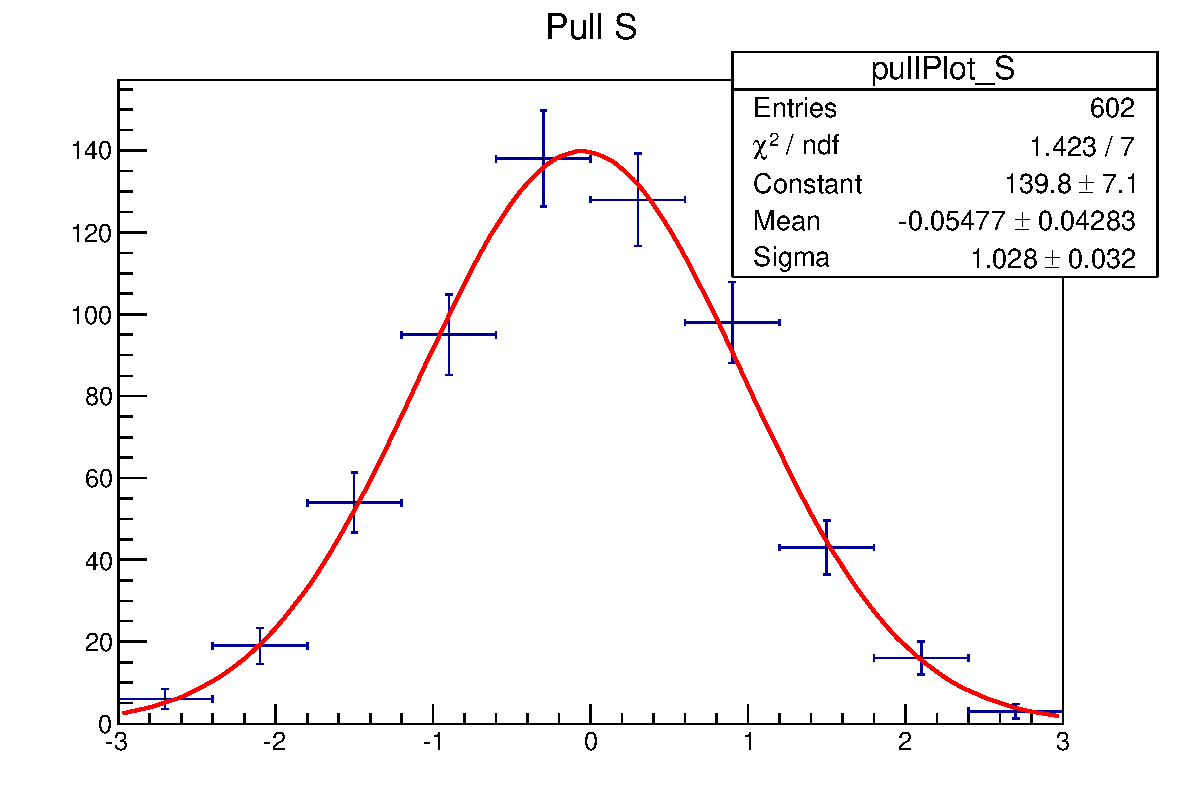
\includegraphics[height=!,width=0.49\textwidth]{figs/plots_toy/studies_timeFit/pull_S_all_Gaussfit.pdf}
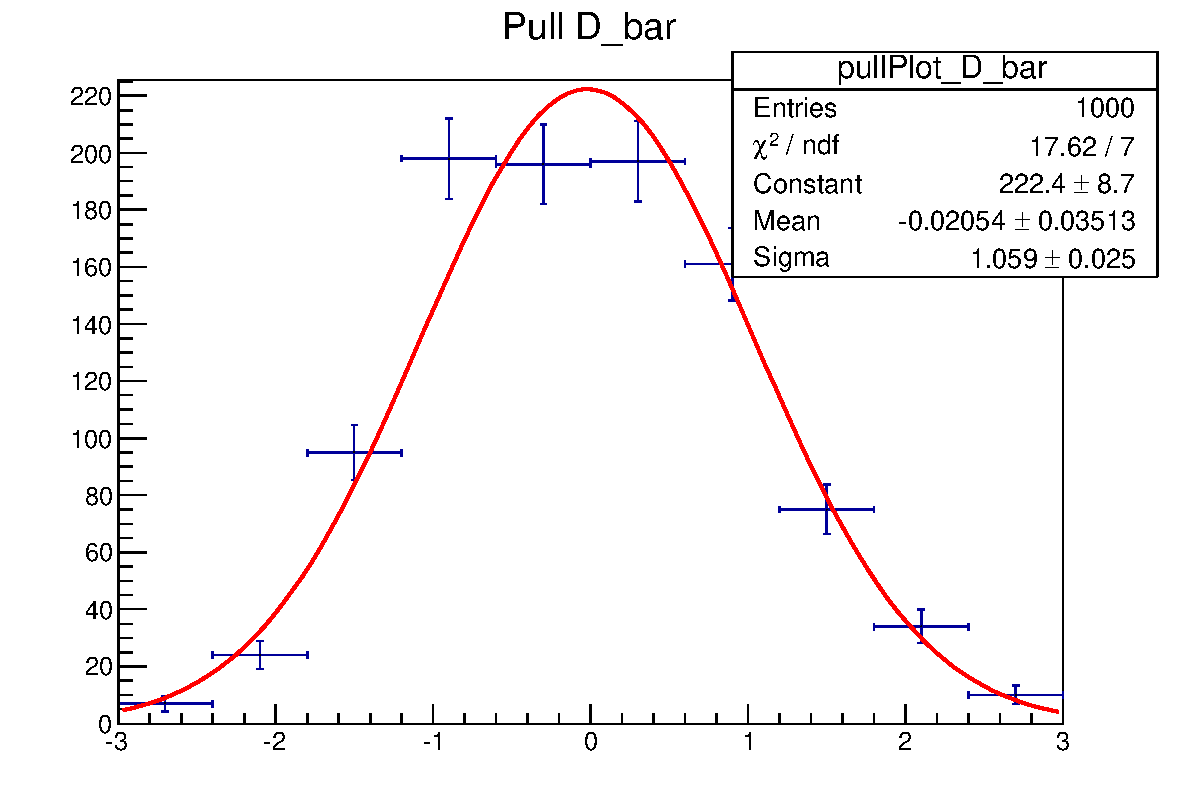
\includegraphics[height=!,width=0.49\textwidth]{figs/plots_toy/studies_timeFit/pull_D_bar_all_Gaussfit.pdf}
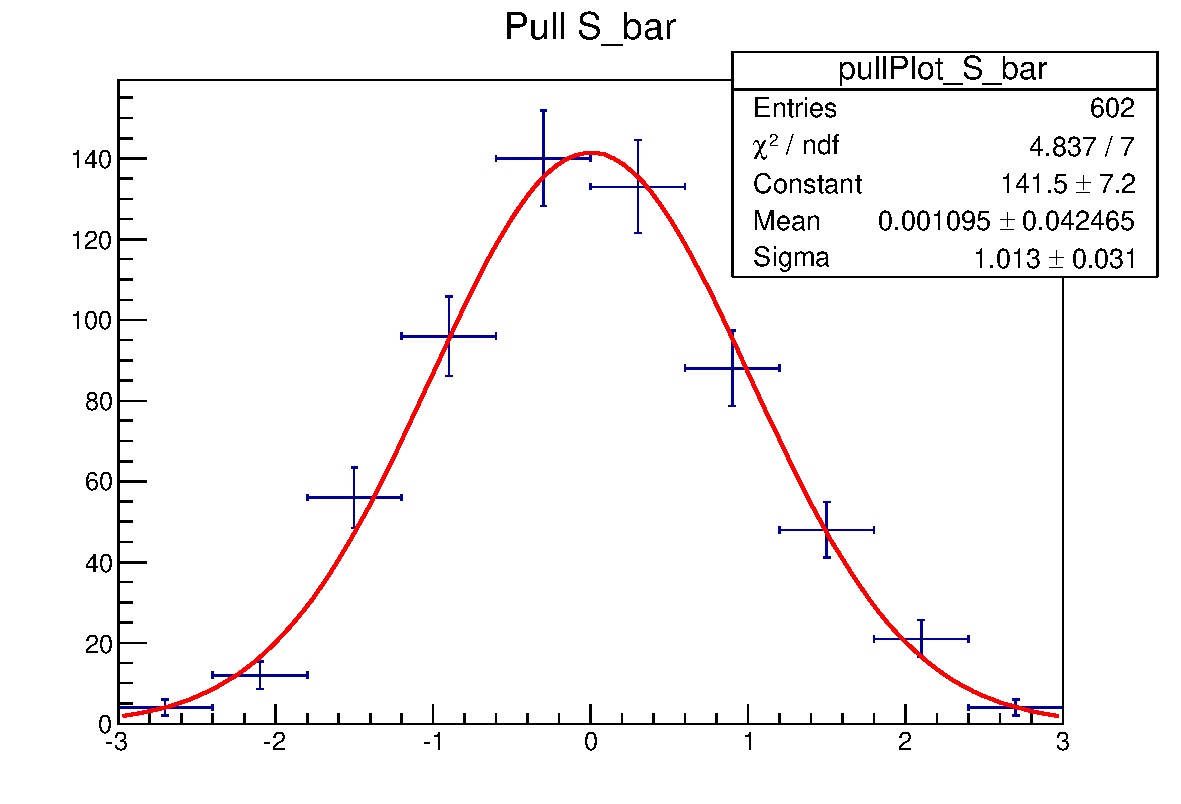
\includegraphics[height=!,width=0.49\textwidth]{figs/plots_toy/studies_timeFit/pull_S_bar_all_Gaussfit.pdf}
\caption{Pull distributions from toy studies for the time-dependent fit, done with 1000 pseudo experiments.}
\label{fig:ToyPulls_tdfit}
\end{figure}


\begin{table}[hp!]
\centering
\caption{Pull parameters for CP coefficients from the toy studies for the time-dependent fit.}
\begin{tabular}{l | c | c}
\hline
Parameter & $\mu$ of pull distribution & $\sigma$ of pull distribution \\
\hline
\hline
C & 0.0344147 $\pm$ 0.0424816 & 1.01956 $\pm$ 0.033269 \\
D & -0.0195562 $\pm$ 0.0431762 & 1.0218 $\pm$ 0.031551 \\
S & -0.0547728 $\pm$ 0.0428276 & 1.02791 $\pm$ 0.0318385 \\
$\bar{D}$ & -0.0173495 $\pm$ 0.0469972 & 1.09866 $\pm$ 0.035404 \\
$\bar{S}$ & 0.00109528 $\pm$ 0.0424655 & 1.01306 $\pm$ 0.0313123 \\
\hline
\end{tabular}
\label{table:Pulls_tDFit}
\end{table}


Table \ref{table:Pulls_tDFit} summarizes the means $\mu$ and widths $\sigma$ of these pull distributions.

